
% LaTeX Beamer file automatically generated from Doconce
% http://code.google.com/p/doconce

%-------------------- begin preamble ----------------------

\documentclass{beamer}

\usetheme{default}
\usecolortheme{default}

% turn off the almost invisible, yet disturbing, navigation symbols:
\setbeamertemplate{navigation symbols}{}

% Examples on customization:
%\usecolortheme[named=RawSienna]{structure}
%\usetheme[height=7mm]{Rochester}
%\setbeamerfont{frametitle}{family=\rmfamily,shape=\itshape}
%\setbeamertemplate{items}[ball]
%\setbeamertemplate{blocks}[rounded][shadow=true]
%\useoutertheme{infolines}
%
%\usefonttheme{}
%\useinntertheme{}
%
%\setbeameroption{show notes}
%\setbeameroption{show notes on second screen=right}

% fine for B/W printing:
%\usecolortheme{seahorse}

\usepackage{pgf,pgfarrows,pgfnodes,pgfautomata,pgfheaps,pgfshade}
\usepackage{graphicx}
\usepackage{epsfig}
\usepackage{minted} % requires pygments and latex -shell-escape filename
\usepackage{fancyvrb,relsize}
\usepackage{amsmath,amssymb,bm}
%\usepackage[latin1]{inputenc}
\usepackage[utf8]{inputenc}
\usepackage{colortbl}
\usepackage[english]{babel}
\usepackage{tikz}
\usepackage{framed,anslistings}
% Use some nice templates
\beamertemplatetransparentcovereddynamic

% Delete this, if you do not want the table of contents to pop up at
% the beginning of each section:
\AtBeginSection[]
{
    \begin{frame}<beamer>[plain]
    \frametitle{}
    \tableofcontents[currentsection]
    \end{frame}
}

% Delete this, if you do not want the table of contents to pop up at
% the beginning of each section:
\AtBeginSection[]
{
    \begin{frame}<beamer>[plain]
    \frametitle{}
    \tableofcontents[currentsection]
    \end{frame}
}

% If you wish to uncover everything in a step-wise fashion, uncomment
% the following command:

%\beamerdefaultoverlayspecification{<+->}

\newcommand{\shortinlinecomment}[3]{\note{\textbf{#1}: #2}}
\newcommand{\longinlinecomment}[3]{\shortinlinecomment{#1}{#2}{#3}}

\newenvironment{notice_colors1admon}[1][]{\begin{block}{#1}}{\end{block}}
\newenvironment{notice_colors2admon}[1][]{\begin{block}{#1}}{\end{block}}
\newenvironment{notice_graybox3admon}[1][]{\begin{block}{#1}}{\end{block}}
\newenvironment{notice_yellowboxadmon}[1][]{\begin{block}{#1}}{\end{block}}
\newenvironment{summary_colors1admon}[1][]{\begin{block}{#1}}{\end{block}}
\newenvironment{summary_colors2admon}[1][]{\begin{block}{#1}}{\end{block}}
\newenvironment{summary_graybox3admon}[1][]{\begin{block}{#1}}{\end{block}}
\newenvironment{summary_yellowboxadmon}[1][]{\begin{block}{#1}}{\end{block}}
\newenvironment{warning_colors1admon}[1][]{\begin{block}{#1}}{\end{block}}
\newenvironment{warning_colors2admon}[1][]{\begin{block}{#1}}{\end{block}}
\newenvironment{warning_graybox3admon}[1][]{\begin{block}{#1}}{\end{block}}
\newenvironment{warning_yellowboxadmon}[1][]{\begin{block}{#1}}{\end{block}}
\newenvironment{question_colors1admon}[1][]{\begin{block}{#1}}{\end{block}}
\newenvironment{question_colors2admon}[1][]{\begin{block}{#1}}{\end{block}}
\newenvironment{question_graybox3admon}[1][]{\begin{block}{#1}}{\end{block}}
\newenvironment{question_yellowboxadmon}[1][]{\begin{block}{#1}}{\end{block}}
\newenvironment{block_colors1admon}[1][]{\begin{block}{#1}}{\end{block}}
\newenvironment{block_colors2admon}[1][]{\begin{block}{#1}}{\end{block}}
\newenvironment{block_graybox3admon}[1][]{\begin{block}{#1}}{\end{block}}
\newenvironment{block_yellowboxadmon}[1][]{\begin{block}{#1}}{\end{block}}
\newenvironment{paragraphadmon}[1][]{\begin{block}{#1}}{\end{block}}
\newenvironment{graybox1admon}[1][]{\begin{block}{#1}}{\end{block}}
\newenvironment{graybox2admon}[1][]{\begin{block}{#1}}{\end{block}}
\newcommand{\grayboxhrules}[1]{\begin{block}{}#1\end{block}}


\newenvironment{exercise}{}{}
\newcounter{exerno}


% insert custom LaTeX commands...

\makeindex

%-------------------- end preamble ----------------------

\begin{document}


\renewcommand{\u}{\pmb{u}}

\newcommand{\xbm}{\bm{x}}
\newcommand{\normalvecbm}{\bm{n}}
\newcommand{\ubm}{\bm{u}}


\newcommand{\x}{\pmb{x}}
\newcommand{\normalvec}{\pmb{n}}
\newcommand{\Ddt}[1]{\frac{D#1}{dt}}
\newcommand{\halfi}{1/2}
\newcommand{\half}{\frac{1}{2}}
\newcommand{\report}{test report}


% ------------------- main content ----------------------



% ----------------- title -------------------------
\title{Test slide features}

% ----------------- author(s) -------------------------
\author{Core Dump\inst{1}}
\institute{Cyber Space Ltd\inst{1}}
% ----------------- end author(s) -------------------------


\date{Jun 29, 2013
\\ \ \\ 
\centerline{
\includegraphics[width=0.5\linewidth]{../doc/slides/fig/doconce1b.png}}
}




\begin{frame}[plain,fragile]
\titlepage
\end{frame}

\begin{frame}[plain,fragile]
\frametitle{Scientific writing for the future needs to address many new media}

\begin{columns}
\column{0.4\textwidth}
\begin{center}  % inline figure
  \centerline{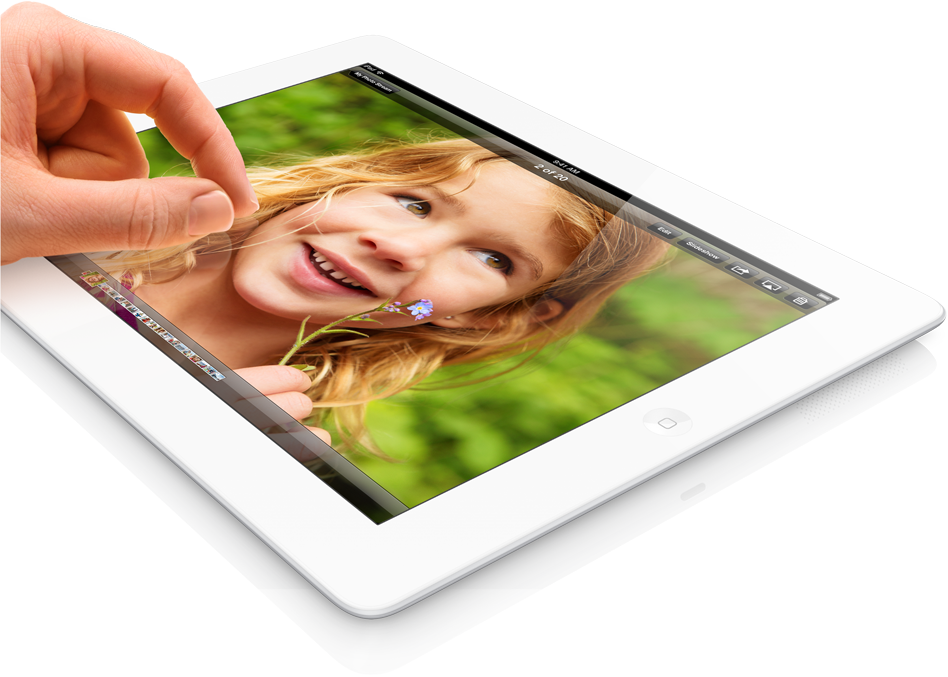
\includegraphics[width=0.8\linewidth]{../doc/slides/fig/ipad.png}}
\end{center}



\begin{center}  % inline figure
  \centerline{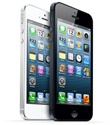
\includegraphics[width=0.3\linewidth]{../doc/slides/fig/iphones.jpg}}
\end{center}


% FIGURE: [../doc/slides/fig/mbair, width=400]


\column{0.6\textwidth}
\begin{center}  % inline figure
  \centerline{
\includegraphics[width=0.7\linewidth]{../doc/slides/fig/imac.png}}
\end{center}


\end{columns}
\end{frame}

\begin{frame}[plain,fragile]
\frametitle{The book will probably survive}

\begin{center}  % inline figure
  \centerline{
\includegraphics[width=0.9\linewidth]{../doc/slides/fig/oldbooks.jpg}}
\end{center}
\end{frame}

\begin{frame}[plain,fragile]
\frametitle{The classical report will survive}

\begin{columns}
\column{0.5\textwidth}
\begin{center}  % inline figure
  \centerline{
\includegraphics[width=1.2\linewidth]{../doc/slides/fig/latex_thesis.jpg}}
\end{center}


\column{0.5\textwidth}
\begin{center}  % inline figure
  \centerline{
\includegraphics[width=1.2\linewidth]{../doc/slides/fig/latex_paper1.png}}
\end{center}


\end{columns}
\end{frame}

\begin{frame}[plain,fragile]
\frametitle{Scope}

% * Scientific writing = lecture notes, slides, reports, thesis, books,  ...
% * (Journal papers typeset by journals are out of scope)

\begin{itemize}
  \item<2-> Scope: documents with \textcolor{red}{much} \emph{math} and \emph{computer code}

  \item<3-> Key question: What tools should I use for writing?

  \item<4-> Default answer: {\LaTeX}

  \item<5-> Alternative: MS Word w/math

  \item<6-> Recent popular alternative tools: HTML w/MathJax,
    Sphinx, Markdown, MediaWiki, IPython notebook
\end{itemize}

\noindent

\begin{columns}
\column{0.25\textwidth}
\begin{center}  % inline figure
  \centerline{
\includegraphics[width=0.3\linewidth]{../doc/slides/fig/LaTeX_logo.jpg}}
\end{center}


\column{0.25\textwidth}
\begin{center}  % inline figure
  \centerline{
\includegraphics[width=0.2\linewidth]{../doc/slides/fig/MS_Word_logo.jpg}}
\end{center}


\column{0.5\textwidth}
\begin{center}  % inline figure
  \centerline{
\includegraphics[width=0.4\linewidth]{../doc/slides/fig/sphinx_logo.png}}
\end{center}


\end{columns}
\begin{columns}
\column{0.25\textwidth}
\begin{center}  % inline figure
  \centerline{
\includegraphics[width=0.2\linewidth]{../doc/slides/fig/markdown_logo.jpg}}
\end{center}


\column{0.25\textwidth}
\begin{center}  % inline figure
  \centerline{
\includegraphics[width=0.2\linewidth]{../doc/slides/fig/MediaWiki_logo.jpg}}
\end{center}


\column{0.5\textwidth}
\begin{center}  % inline figure
  \centerline{
\includegraphics[width=0.6\linewidth]{../doc/slides/fig/IPython_logo.png}}
\end{center}


\end{columns}
\end{frame}

\begin{frame}[plain,fragile]
\frametitle{Scientific writing for the future needs to address many new media}

% Insert links here to reports

\begin{columns}
\column{0.5\textwidth}
Old days (1985-2005): {\LaTeX} for BW paper output, but now

\begin{enumerate}
  \item BW books

  \item Colorful PDF books (printed and screen)

  \item Designed web pages

  \item Wikis

  \item Bloggs

  \item Next new fancy format (iBook w/LaTeX?)
\end{enumerate}

\noindent

\column{0.5\textwidth}
\begin{center}  % inline figure
  \centerline{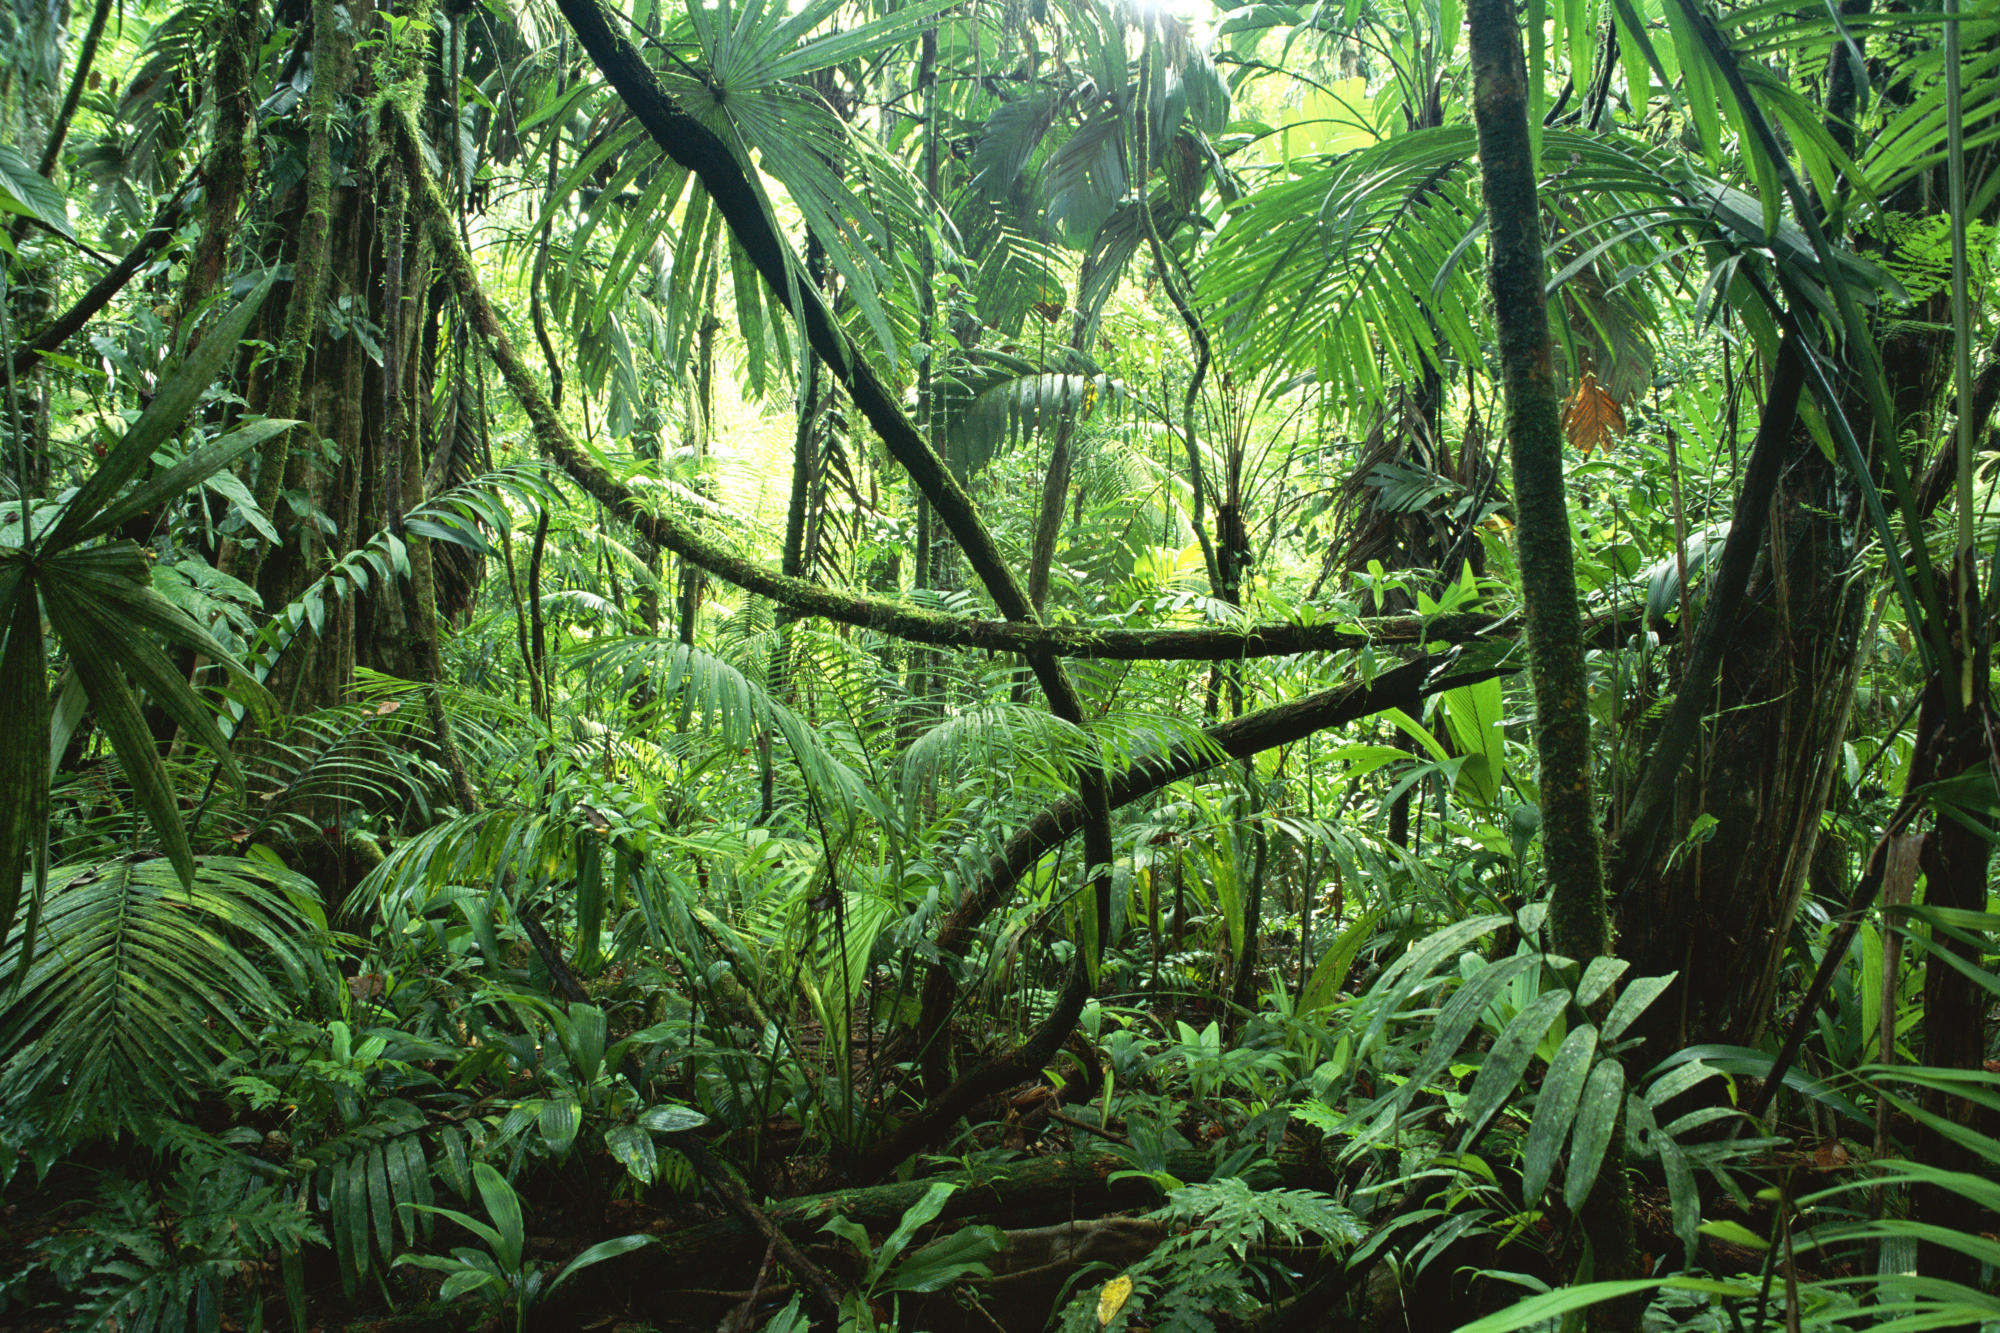
\includegraphics[width=0.9\linewidth]{../doc/slides/fig/jungle_with_mess.jpg}}
\end{center}


\end{columns}
\end{frame}

\begin{frame}[plain,fragile]
\frametitle{Fundamental question}

When I write some scientific material,

\begin{itemize}
 \item a {\LaTeX} document,

 \item a blogg (HTML),

 \item some web pages (HTML),

 \item a Sphinx document,

 \item some Markdown files,
\end{itemize}

\noindent
and later want to collect the pieces into a larger document, maybe
some book, or one big web document, is that at all feasible?


\pause
\begin{block}{}
Probably not, but I have a solution :-)
\end{block}
\end{frame}

\begin{frame}[plain,fragile]
\frametitle{{\LaTeX}

is very rich; other tools support only some elements}

\begin{itemize}
 \item {\LaTeX} inline math: works with all ({\LaTeX}, MathJax, Sphinx, Markdown, MediaWiki)

 \item {\LaTeX} equation math:
\begin{itemize}

    \item \textbf{LaTeX}: \Verb!equation*!, \Verb!equation!, \Verb!align*!, \Verb!align! +
      \Verb!eqnarray!, \Verb!split!, \Verb!alignat!, ... (numerous!)

    \item \textbf{MathJax}: \Verb!equation*!, \Verb!equation!, \Verb!align*!, \Verb!align!

    \item \textbf{MediaWiki}: \Verb!equation*!, \Verb!equation!, \Verb!align*!, \Verb!align!

    \item \textbf{Sphinx}: \Verb!equation*!, \Verb!equation!, \Verb!align*!

    \item \textbf{Markdown}: \Verb!equation*!, \Verb!equation!, \Verb!eqnarray*!, \Verb!align*! (but no labels)
\end{itemize}

\noindent
\end{itemize}

\noindent
\end{frame}

\begin{frame}[plain,fragile]
\frametitle{{\LaTeX}

is very rich; other tools support only some elements}


\pause
\begin{block}{}
\begin{itemize}
 \item Figures: all

 \item Subfigures: {\LaTeX} (\Verb!subfigure!)

 \item Movies: {\LaTeX} (can run separately), just raw embedded HTML in others

 \item Floating computer code: {\LaTeX}

 \item Fixed computer code: all

 \item Floating tables: {\LaTeX}; inline tables: all

 \item Algorithms: {\LaTeX}

 \item Margin notes: {\LaTeX}

 \item Page references: {\LaTeX}

 \item Footnotes: {\LaTeX}, Sphinx, reStructuredText, MediaWiki

 \item Bibliography: {\LaTeX}, Sphinx, reStructuredText, MediaWiki

 \item Hyperlinks: all (but not on paper!)
\end{itemize}

\noindent
\end{block}



\pause
\begin{block}{}
Conclusion: Highly non-trivial to translate a {\LaTeX} document into something
based on HTML and vice versa.
\end{block}
\end{frame}

\begin{frame}[plain,fragile]
\frametitle{Doconce demo}

\href{{http://hplgit.github.com/teamods/writing_reports/}}{\nolinkurl{http://hplgit.github.com/teamods/writing_reports/}}

\begin{itemize}
 \item LaTeX-based PDF \href{{http://hplgit.github.com/teamods/writing_reports/_static/report.pdf}}{for screen}, \href{{http://hplgit.github.com/teamods/writing_reports/_static/report_4printing.pdf}}{for printing}, \href{{http://hplgit.github.com/teamods/writing_reports/_static/report_4phone.pdf}}{for phone}

 \item \href{{http://hplgit.github.com/teamods/writing_reports/_static/report_do.html}}{Plain HTML} or with a \href{{http://hplgit.github.com/teamods/writing_reports/_static/report_vagrant.html}}{template} or \href{{http://hplgit.github.com/teamods/writing_reports/_static/report_github_minimal.html}}{another template} or \href{{http://hplgit.github.com/teamods/writing_reports/_static/report_solarized.html}}{solarized}

 \item Sphinx: \href{{http://hplgit.github.com/teamods/writing_reports/_static/sphinx-agni/index.html}}{agni}, \href{{http://hplgit.github.com/teamods/writing_reports/_static/sphinx-pyramid/report.html}}{pyramid}, \href{{http://hplgit.github.com/teamods/writing_reports/_static/sphinx-classy/report.html}}{classy}, \href{{http://hplgit.github.com/teamods/writing_reports/_static/sphinx-fenics_minimal/report.html}}{fenics}, \href{{http://hplgit.github.com/teamods/writing_reports/_static/sphinx-fenics_minimal/report.html}}{redcloud}

 \item HTML for \href{{http://doconce-report-demo.blogspot.no/}}{Google} or \href{{http://doconcereportdemo.wordpress.com/}}{Wordpress} blogs

 \item \href{{http://doconcedemo.shoutwiki.com/wiki/Doconce_demo_page}}{MediaWiki} (Wikipedia, Wikibooks, etc)

 \item Doconce \href{{http://hplgit.github.com/teamods/writing_reports/_static/report.do.txt.html}}{source code} and \href{{http://code.google.com/p/doconce/wiki/Tutorial}}{tutorial}
\end{itemize}

\noindent
\end{frame}

\begin{frame}[plain,fragile]
\frametitle{A tour of Doconce}

% latex interprets 9 = as chapter and then needs book style...
\end{frame}

\begin{frame}[plain,fragile]
\frametitle{Doconce: title, authors, date, toc}

\begin{Verbatim}[numbers=none,fontsize=\fontsize{9pt}{9pt},baselinestretch=0.95]
TITLE: Some Title
AUTHOR: name1 at institution1, with more info, and institution2
AUTHOR: name2 email:name2@web.com at institution
DATE: today

# A table of contents is optional:
TOC: on
\end{Verbatim}


\begin{graybox1admon}[Notice.]
Title and authors must have all information \emph{on a single line}!
\end{graybox1admon}
\end{frame}

\begin{frame}[plain,fragile]
\frametitle{Doconce: abstract}

\begin{Verbatim}[numbers=none,fontsize=\fontsize{9pt}{9pt},baselinestretch=0.95]
__Abstract.__
Here goes the abstract...
\end{Verbatim}

Or:
\begin{Verbatim}[numbers=none,fontsize=\fontsize{9pt}{9pt},baselinestretch=0.95]
__Summary.__
Here goes the summary...
\end{Verbatim}
\end{frame}

\begin{frame}[plain,fragile]
\frametitle{Doconce: section headings}

Headings are surrounded by \Verb!=! signs:
\begin{Verbatim}[numbers=none,fontsize=\fontsize{9pt}{9pt},baselinestretch=0.95]
========= This is an H1/chapter heading =========

======= This is an H2/section heading =======

===== This is an H3/subsection heading =====

=== This is an H4/paragraph heading ===

__This is a paragraph heading.__
\end{Verbatim}

Result:

\noindent\textbf{\huge This is an H1/chapter heading}

\noindent\textbf{\Large This is an H2/section heading}

\noindent\textbf{\large This is an H3/subsection heading}

\noindent\textbf{This is an H4/paragraph heading.}
\noindent\textbf{This is a paragraph heading.}
\end{frame}

\begin{frame}[plain,fragile]
\frametitle{Doconce: markup and lists}

\begin{Verbatim}[numbers=none,fontsize=\fontsize{9pt}{9pt},baselinestretch=0.95]
 * Bullet list items start with `*`
   and may span several lines
 * *Emphasized words* are possible
 * _Boldface words_ are also possible
 * color{red}{colored words} too
 * `inline verbatim code` is featured
   o and sublists with enumerated items starting with `o`
   o items are just indented as you would do in email
\end{Verbatim}

This gets rendered as

\begin{itemize}
 \item Bullet lists start with \Verb!*!
   and may span several lines

 \item \emph{Emphasized words} are possible

 \item \textbf{Boldface words} are also possible

 \item \textcolor{red}{colored words} too

 \item \Verb!inline verbatim code! is featured
\begin{enumerate}

  \item and sublists with enumerated items starting with \Verb!o!

  \item items are just indented as you would do in email
\end{enumerate}

\noindent
\end{itemize}

\noindent
\end{frame}

\begin{frame}[plain,fragile]
\frametitle{Doconce: labels, references, index items}

\begin{Verbatim}[numbers=none,fontsize=\fontsize{9pt}{9pt},baselinestretch=0.95]
# Insert index items in the source
idx{key word1} idx{key word2}

# Label
===== Some section =====
label{this:section}

# Make reference
As we saw in Section ref{this:section}, references, index
items and labels follow a syntax similar to LaTeX
but without backslashes.

# Make reference to equations
See (ref{eq1})-(ref{myeq}).

# Make hyperlink
"some link text": "http://code.google.com/p/doconce/"

# Hyperlink with complete URL as link text
URL: "http://code.google.com/p/doconce/"
\end{Verbatim}
\end{frame}

\begin{frame}[plain,fragile]
\frametitle{Doconce: figures and movies}

\begin{graybox1admon}[Notice.]
Figure with HTML and {\LaTeX} info, and caption, \emph{all on one line}:
\end{graybox1admon}

\begin{Verbatim}[numbers=none,fontsize=\fontsize{9pt}{9pt},baselinestretch=0.95]
FIGURE: [figdir/myfig, width=300 frac=1.2] My caption. label{fig1}

# This figure will be 300 pixels wide in HTML and span 1.2 times
# the linewidth in LaTeX.
\end{Verbatim}

Movies are also supported:

\begin{Verbatim}[numbers=none,fontsize=\fontsize{9pt}{9pt},baselinestretch=0.95]
MOVIE: [http://www.youtube.com/embed/P8VcZzgdfSc, width=420 height=315]
\end{Verbatim}
and rendered as

 \href{{http://www.youtube.com/watch?v=P8VcZzgdfSc}}{\nolinkurl{http://www.youtube.com/watch?v=P8VcZzgdfSc}}
\end{frame}

\begin{frame}[plain,fragile]
\frametitle{Doconce: math}

Inline math as in {\LaTeX}:

\begin{Verbatim}[numbers=none,fontsize=\fontsize{9pt}{9pt},baselinestretch=0.95]
...where $a=\int_{\Omega}fdx$ is an integral.
\end{Verbatim}
gets rendered as ...where $a=\int_{\Omega}fdx$ is an integral.


An equation environment is surrounded by \Verb!!bt! and \Verb!!et! tags,
the rest is plain {\LaTeX}:

\begin{Verbatim}[numbers=none,fontsize=\fontsize{9pt}{9pt},baselinestretch=0.95]
!bt
\begin{align}
\frac{\partial u}{\partial t} &= \nabla^2 u,
label{a:eq}\\
\nabla\cdot\pmb{v} & = 0
label{b:eq}
\end{align}
!et
\end{Verbatim}
which is rendered as

\begin{align}
\frac{\partial u}{\partial t} &= \nabla^2 u,
\label{a:eq}\\
\nabla\cdot\pmb{v} & = 0
\label{b:eq}
\end{align}
\end{frame}

\begin{frame}[plain,fragile]
\frametitle{Doconce: displaying code}

Code is enclosed in \Verb!!bc! and \Verb!!ec! tags:

\begin{Verbatim}[numbers=none,fontsize=\fontsize{9pt}{9pt},baselinestretch=0.95]
!bc pycod
def solver(I, a, T, dt, theta):
    """Solve u'=-a*u, u(0)=I, for t in (0,T] with steps of dt."""
    dt = float(dt)           # avoid integer division
    N = int(round(T/dt))     # no of time intervals
    T = N*dt                 # adjust T to fit time step dt
    u = zeros(N+1)           # array of u[n] values
    t = linspace(0, T, N+1)  # time mesh

    u[0] = I                 # assign initial condition
    for n in range(0, N):    # n=0,1,...,N-1
        u[n+1] = (1 - (1-theta)*a*dt)/(1 + theta*dt*a)*u[n]
    return u, t
!ec
\end{Verbatim}
This gets rendered as

\begin{minted}[fontsize=\fontsize{9pt}{9pt},linenos=false,mathescape,baselinestretch=1.0,fontfamily=tt,xleftmargin=7mm]{python}
def solver(I, a, T, dt, theta):
    """Solve u'=-a*u, u(0)=I, for t in (0,T] with steps of dt."""
    dt = float(dt)           # avoid integer division
    N = int(round(T/dt))     # no of time intervals
    T = N*dt                 # adjust T to fit time step dt
    u = zeros(N+1)           # array of u[n] values
    t = linspace(0, T, N+1)  # time mesh

    u[0] = I                 # assign initial condition
    for n in range(0, N):    # n=0,1,...,N-1
        u[n+1] = (1 - (1-theta)*a*dt)/(1 + theta*dt*a)*u[n]
    return u, t
\end{minted}


\begin{graybox1admon}[Language-dependent typesetting of code:]
The \Verb!!bc! command can be followed by a specification of the computer
language: \Verb!pycod! for Python code snippet, \Verb!pypro! for complete Python
program, \Verb!fcod! for Fortran snippet, \Verb!fpro! for Fortran program, and so
forth (\Verb!c! for C, \Verb!cpp! for C++, \Verb!sh! for Unix shells, \Verb!m! for Matlab).
\end{graybox1admon}
\end{frame}

\begin{frame}[plain,fragile]
\frametitle{Doconce: displaying interactive demo code}

\label{slide:pot}

With \Verb!!bc pyoptpro! or a file \Verb!*.pyopt!, the code applies the
\href{{http://pythontutor.com}}{Online Python Tutor} for displaying
program flow and state of variables:

\begin{minted}[fontsize=\fontsize{9pt}{9pt},linenos=false,mathescape,baselinestretch=1.0,fontfamily=tt,xleftmargin=7mm]{python}
def solver(I, a, T, dt, theta):
    dt = float(dt)
    N = int(round(T/dt))
    T = N*dt
    u = [0.0]*(N+1)
    t = [i*dt for i in range(N+1)]

    u[0] = I
    for n in range(0, N):
        u[n+1] = (1 - (1-theta)*a*dt)/(1 + theta*dt*a)*u[n]
    return u, t

u, t = solver(I=1, a=1, T=3, dt=1., theta=0.5)
print u
\end{minted}
\noindent
(\href{{http://pythontutor.com/visualize.html\#code=def+solver\%28I\%2C+a\%2C+T\%2C+dt\%2C+theta\%29\%3A\%0A++++dt+\%3D+float\%28dt\%29\%0A++++N+\%3D+int\%28round\%28T\%2Fdt\%29\%29\%0A++++T+\%3D+N\%2Adt\%0A++++u+\%3D+\%5B0.0\%5D\%2A\%28N\%2B1\%29\%0A++++t+\%3D+\%5Bi\%2Adt+for+i+in+range\%28N\%2B1\%29\%5D\%0A\%0A++++u\%5B0\%5D+\%3D+I\%0A++++for+n+in+range\%280\%2C+N\%29\%3A\%0A++++++++u\%5Bn\%2B1\%5D+\%3D+\%281+-+\%281-theta\%29\%2Aa\%2Adt\%29\%2F\%281+\%2B+theta\%2Adt\%2Aa\%29\%2Au\%5Bn\%5D\%0A++++return+u\%2C+t\%0A\%0Au\%2C+t+\%3D+solver\%28I\%3D1\%2C+a\%3D1\%2C+T\%3D3\%2C+dt\%3D1.\%2C+theta\%3D0.5\%29\%0Aprint+u&mode=display&cumulative=false&heapPrimitives=false&drawParentPointers=false&textReferences=false&py=2&curInstr=0}}{Visualize execution})
\end{frame}

\begin{frame}[plain,fragile]
\frametitle{Doconce: exercises}

Doconce offers a special format for \emph{exercises}, \emph{problems}, \emph{projects},
and \emph{examples}:

\begin{Verbatim}[numbers=none,fontsize=\fontsize{9pt}{9pt},baselinestretch=0.95]
===== Problem: Flip a Coin =====
label{demo:ex:1}

files = flip_coin.py, flip_coin.pdf
solutions = mysol.txt, mysol_flip_coin.py
keywords = random numbers; Monte Carlo simulation

!bsubex
Make a program that simulates flipping a coin $N$ times.

\noindent\textbf{Hint.}\n
Use `r = random.random()` and define head as `r <= 0.5`.

!esubex

!bsubex
Compute the probability of getting heads.

!bans
A short answer: 0.5.
!eans

!bsol
A full solution to this subexercise can go here.
!esol
!esubex

!bsubex
Make another program that computes the probability
of getting at least three heads out of 5 throws.
!esubex
\end{Verbatim}

Solutions/answers can easily be left out of the document.
\end{frame}

\begin{frame}[plain,fragile]
\frametitle{Doconce: exercises}

Last page gets rendered as follows:



% --- begin exercise ---
\begin{exercise}
\refstepcounter{exerno}

\subsection*{Problem 1: Flip a Coin}
\label{demo:ex:1}
% keywords = random numbers; Monte Carlo simulation


\noindent\textbf{a)}
Make a program that simulates flipping a coin $N$ times.

% --- begin hint in exercise ---

\noindent\textbf{Hint.}
Use \Verb!r = random.random()! and define head as \Verb!r <= 0.5!.
% --- end hint in exercise ---

\noindent\textbf{b)}
Compute the probability of getting heads.


% --- begin answer of exercise ---
\noindent\textbf{Answer.}
A short answer: 0.5.
% --- end answer of exercise ---


% --- begin solution of exercise ---
\noindent\textbf{Solution.}
A full solution to this subexercise can go here.
% --- end solution of exercise ---

\noindent\textbf{c)}
Make another program that computes the probability
of getting at least three heads out of 5 throws.

Filenames: \Verb!flip_coin.py!, \Verb!flip_coin.pdf!.
% solution files: mysol.txt, mysol_flip_coin.py

\end{exercise}
% --- end exercise ---
\end{frame}

\begin{frame}[plain,fragile]
\frametitle{Doconce: example on slide code}

\begin{Verbatim}[numbers=none,fontsize=\fontsize{9pt}{9pt},baselinestretch=0.95]
!split
======= Headline =======

 * Key point 1
 * Key point 2
 * Key point 3 takes very much more text to explain because
   this point is really comprehensive, and although long
   bullet points are not recommended in general, we need
   it here for demonstration purposes

FIGURE: [../doc/slides/fig/teacher1, width=100]

Key equation:

!bt
\[ -\nabla^2 u = f \quad\hbox{in }\Omega \]
!et

And maybe a final comment?

!split
======= Next slide... =======
\end{Verbatim}
\end{frame}

\begin{frame}[plain,fragile]
\frametitle{Doconce: example on slide code}

Last page gets rendered to

\noindent\textbf{\Large Headline}

\begin{itemize}
 \item Key point 1

 \item Key point 2
\end{itemize}

\noindent
\begin{center}  % inline figure
  \centerline{
\includegraphics[width=0.4\linewidth]{../doc/slides/fig/teacher1.pdf}}
\end{center}


Key equation:

\[ -\nabla^2 u = f \quad\hbox{in }\Omega \]

And maybe a final comment?
\end{frame}

\begin{frame}[plain,fragile]
\frametitle{Doconce: example on slide code with cells}

One can introduce a table-like layout with MxN cells and
put slide elements in various cell. A cell with position
MN is surrounded by \Verb!!bslidecell MN! and \Verb!!eslidecell!
tags. Below is an example with a bullet list to the left and
a figure to the right (two cells, numbered 00 and 01).

\begin{Verbatim}[numbers=none,fontsize=\fontsize{9pt}{9pt},baselinestretch=0.95]
!split
======= Headline =======

!bslidecell 00
!bpop
 * Key point 1
 * Key point 2
 * Key point 3 takes very much more text to explain because
   this point is really comprehensive, and although long
   bullet points are not recommended in general, we need
   it here for demonstration purposes
!epop

!bpop
!bt
\[ -\nabla^2 u = f \quad\hbox{in }\Omega \]
!et
!epop

!eslidecell

!bslidecell 01
FIGURE: [../doc/slides/fig/broken_pen_and_paper, width=400, frac=0.8]
!eslidecell

!split
======= Next slide... =======
\end{Verbatim}
\end{frame}

\begin{frame}[plain,fragile]
\frametitle{Doconce: example on slide code}

Last page gets rendered to

\noindent\textbf{\Large Headline}

\begin{columns}
\column{0.5\textwidth}

\pause
\begin{block}{}
\begin{itemize}
 \item Key point 1

 \item Key point 2

 \item Key point 3 takes very much more text to explain because
   this point is really comprehensive, and although long
   bullet points are not recommended in general, we need
   it here for demonstration purposes
\end{itemize}

\noindent
\end{block}



\pause
\begin{block}{}
\[ -\nabla^2 u = f \quad\hbox{in }\Omega \]
\end{block}



\column{0.5\textwidth}
\begin{center}  % inline figure
  \centerline{
\includegraphics[width=0.9\linewidth]{../doc/slides/fig/broken_pen_and_paper.jpg}}
\end{center}


\end{columns}
\end{frame}

\end{document}
